\subsection{Assignment problem}
\label{assign_problem}

I've found this at \url{http://www.math.harvard.edu/archive/20_spring_05/handouts/assignment_overheads.pdf} and took screenshot:

\begin{figure}[H]
\centering
\frame{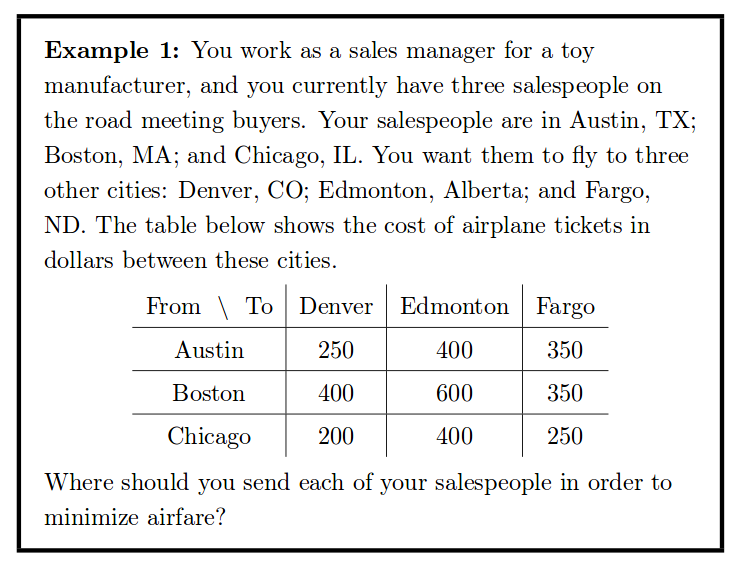
\includegraphics[scale=0.6]{MaxSMT/assign_problem/1.png}}
\end{figure}

As in my previous examples, Z3 and SMT-solver may be overkill for the task.
Simpler algorithm exists for this task (\textit{Hungarian algorithm/method})
\footnote{See also: \url{https://en.wikipedia.org/wiki/Hungarian_algorithm}.}.

But again, I use it to demonstrate the problem + as SMT-solvers demonstration.

Here is what I do:

\lstinputlisting[style=custompy]{MaxSMT/assign_problem/1.py}

In plain English this means \textit{choose such columns, so that their sum would be as small as possible}.

Result is seems to be correct:

\begin{lstlisting}
sat
[choice_0 = 1,
 choice_1 = 2,
 choice_2 = 0,
 z3name!12 = 0,
 z3name!7 = 1,
 z3name!10 = 2,
 z3name!8 = 0,
 z3name!11 = 0,
 z3name!9 = 0,
 final_sum = 950,
 row_value_2 = 200,
 row_value_1 = 350,
 row_value_0 = 400]
\end{lstlisting}

Again, as it is in the corresponding PDF presentation:

\begin{figure}[H]
\centering
\frame{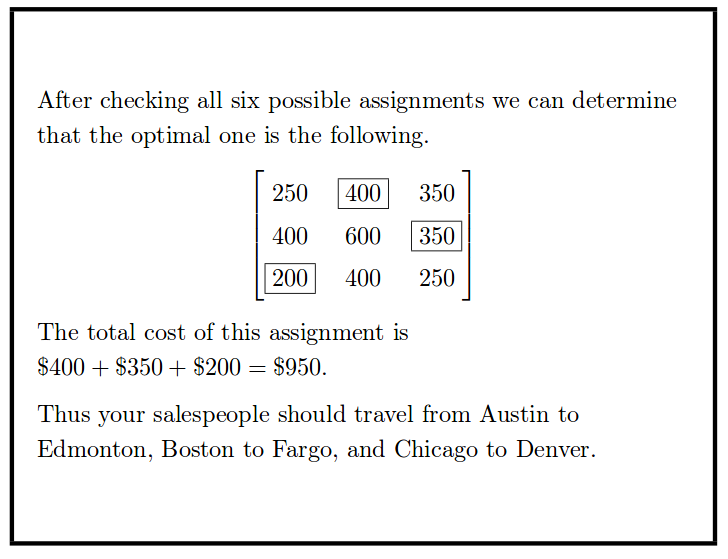
\includegraphics[scale=0.6]{MaxSMT/assign_problem/2.png}}
\end{figure}

(However, I've no idea what ``z3name'' variables mean, perhaps, some internal variables?)\\
\\
The problem can also be stated in SMT-LIB 2.0 format, and solved using MK85:

\lstinputlisting{MaxSMT/assign_problem/assign_problem.smt}

\lstinputlisting[caption=The result]{MaxSMT/assign_problem/assign_problem.correct}

